\documentclass{mcmthesis}
%------------------basic settings-------------------
\mcmsetup{
	CTeX = false,
    tcn = 00000,
    problem = A,
    sheet = true, 
    titleinsheet = true, 
    keywordsinsheet = false,
    titlepage = false, 
    abstract = false
}

\usepackage{indentfirst}
\setlength{\parindent}{2em}
\newcommand{\tabincell}[2]{\begin{tabular}{@{}#1@{}}#2\end{tabular}}


% 正文标题
\title{UESTC\_00 ASC 2018 Proposal}

\def\summarysheetname{Abstract}


%---------------document begin----------------------
\begin{document}

% control sheet ---------->
\begin{summarysheet}
\par This paper presents the corresponding scheme and test results for the four topics of the ASC-2018 contest.
\par First of all, this paper presents the efforts and achievements made by the University of Electronic Science and Technology in supercomputers, and the basic conditions of the participating teams. Then, we presented the HPC platform we designed under the 3000 watt power consumption limit. And we have already Hardware-based HPL and HPCG-based performance tuning. Next, this paper presents optimized parameters and code adjustments for Relion and gives the heaviest results. Finally, we give the neural network we designed forAnswer Prediction for Search Query's Models and results.


\end{summarysheet}

\maketitle
% control sheet over -------------->


% Table of Contents --------------->
\tableofcontents
\newpage

\section{Supercomputing Activities in UESTC}

\subsection{Background}

\par Due to chip power consumption and physical limitations, Moore's Law continues to be effective and results in higher processor performance. The traditional method of increasing the processor frequency has shifted to increasing the number of computing cores. The processor rapidly evolves from single core to multi-core and multiple cores. In fact, mainstream personal processor chips have virtually halted the production of single-core processors since 2007. Commercial CPUs currently on the market usually integrate 4 to 8 computing cores, complemented by the hyper-threading technology provided by the chip manufacturers (such as Intel HT), enabling parallel computation of 8 to 16 physical threads. The introduction of GPGPU products, making the PC's computing power to further strengthen. Computer system architecture has been fully entered the era of multi-core processors from the era of single-core processors.

\par In the multi-core, all-nuclear chip-led consumer market, parallel computing is no longer super-computing proprietary technology. Parallel computing has expanded from the field of supercomputing to traditional business applications and personal information services and has become the core technology to improve the energy efficiency and energy saving of computer programs.

\par Supercomputing is the frontier research field of current computer science and technology, which is a high-level application of parallel computing. It is of strategic importance to the national economy, national security and the progress of science and technology, and is one of the important symbols to measure the overall strength of a country. In the recent ten years, the global supercomputer jumped from ten trillion times to several petaflops, achieving a hundredfold increase in performance. It is estimated that a terabyte-scale supercomputing platform will be built around 2018, which will be 20 times faster than the fastest Tianhe II now in the world to meet the needs of many fields including astrophysics and cosmology, physics and chemistry, life sciences, earth sciences , Systems and Engineering Science in five major areas of science and engineering computing needs.

\subsection{Supercomputing-Related Hardware and Software Platforms}

\subsubsection{Hardware Platforms}

\par Inspur Tiansuo series HPC platform (Show in table \ref{tab:Hardware Platforms in UESTC}).

\begin{table}[h]
\centering
\caption{Hardware Platforms in UESTC}\label{tab:Hardware Platforms in UESTC}
\begin{tabular}{ccc}
\toprule
Device Name &$\qquad \qquad$ & Number\\
\midrule
Inspur TS4220 Cabinet  &$\qquad \qquad$& 1 \\
Inspur S1000KVM Console &$\qquad \qquad$ & 1 \\
NF5280M4 Management Node &$\qquad \qquad$& 1 \\
NF5280M4 GPGPU Compute Node &$\qquad \qquad$& 8 \\
H3C S1224 Gigabit Ethernet Switch &$\qquad \qquad$& 2 \\
Intel Xeon Phi 7120P Coprocessor &$\qquad \qquad$& 6 \\
Nvidia Tesla K80 &$\qquad \qquad$& 4 \\
GForce GTX 780 &$\qquad \qquad$& 6 \\
\bottomrule
\end{tabular}
\end{table}

\newpage

\subsubsection{Software Platforms}

\begin{itemize}
	\item Operating System: RedHat Linux
	\item Development Kit
	\begin{itemize}
		\item Intel C++/Fortran Compiler
		\item Intel MKL Math Core Library
		\item GNU series compiler
	\end{itemize}
	\item Operating environment
	\begin{itemize}
		\item MVAPICH2, OpenMPI and MPICH Parallel Environment
		\item HPC, Hadoop and Spark Computing Environment
	\end{itemize}
	\item Tuning Documentation
	\begin{itemize}
		\item MVAPICH2-X/GDR/MIC,  HPC-X Toolkit, OpenMPI and MPICH2 Parameter Tuning Documentation
		\item ATLAS, ApenBLAS, Lapack, ScalAPACK and FFTW3 Mathematical Library Parameter Tuning Documentation
	\end{itemize}
\end{itemize}


\subsection{Supercomputing-Related Courses, Trainings, and Interest Groups}


\begin{itemize}
	\item Object-Oriented Programming Java: JavaThreads multi-threaded programming.
	\item Operating system, computer network programming: PThreads multi-threaded program development.
	\item Distributed and Parallel Computing, Numerical Analysis, Computational Math Fundamentals: MPI, OpenMP, CUDA Programming, OpenCL Heterogeneous Programming.
	\item CUDA programming: CUDA.
\end{itemize}


\subsection{Supercomputing-Related Research and Applications} 
\par The supercomputing project leader Guoming Lu has more than 10 years of experience in supercomputing and cloud computing. He has led students to participate in college students' supercomputing competitions for many times, and has a deep background in scientific research and teaching in areas related to supercomputing. The other members of the team are also related to distributed computing and data mining. At the same time, the laboratory has completed several research projects and experimental projects in supercomputing and high performance computing. Therefore, the team has a good research in supercomputing. And teaching basis.

\subsubsection{High-level Laboratory planning and construction}

\par Project Leaders successfully applied for NSF "Parallel Distributed Computing Curriculum Innovation Project" and NVIDIA "CUDA Teaching Center" in October 2013 and October 2014, respectively, through experts in the field of supercomputing and world-class GPUs. Hardware manufacturers communicate and communicate to ensure a high level of laboratory planning and experimental design.

\subsubsection{Supercomputing Laboratory Service College Sudent Competition}

\par As a supercomputing laboratory, the supernumerary competition for students has been trained and occupied. The laboratory is committed to greatly improving the college students' supercomputing level, which will enable UESTC to occupy a place in the international arena of the supercomputing competition.

\subsubsection{Teaching and Scientific Research Promote Each Other}

\par Through the supercomputing lab, a school's own supercomputing experimental computing platform, service computer college, and other colleges' supercomputing requirements were established. During the process of in-depth scientific research, extensive application cases were collected, and the supercomputing experiment was extensively explored and enriched. Achieve mutual promotion of scientific research and teaching.


\subsection{The Key Achievements on Supercomputing Education}

\subsubsection{Our HPC Education Development Process}
\par Our school of computer science in the response to the trend of computer parallel professional training program to adjust in most domestic colleges and universities in front of. In 2010, the School of Computer Science and Technology of the UESTC revised the program of computer science (undergraduate) training and opened the "distributed parallel computing" course (the seventh semester) at the 2010 training program to adapt to the traditional training of multicore and parallel computing technologies Program challenges. In October 2013, as the third university in mainland China, UESTC successfully joined the American NSF "Parallel Distributed Computing Curriculum Innovation Project", initiated the curriculum reform of computer science and technology, and began to strengthen the overall reform of professional courses. Parallel computing is taught in various courses in computer science and technology. The project initially covered four topics: Computer Architecture, Computer Network Programming, Java Programming Language Design and New Open Course Distributed and Parallel Computing, focusing on the research of distributed parallel computing knowledge points in the course group Reasonable distribution, to help students from hardware to software to establish the concept of distributed parallel computing, to help students adapt to the development trend of computer parallelism. At present, distributed parallel computing courses were first taught to seniors in the fall of 2013 and were well received by students. According to the results of the pre-course reform, the School of Computer Science put forward that the three courses of algorithm and data structure, operating system and compilation principle are also included in the teaching reform curriculum group so as to provide students with comprehensive knowledge of distributed parallel computing and establish complete knowledge of parallel computing system. In October 2014, the course reform program was once again nominated for NSF's "Parallel Distributed Computing Curriculum Innovation Project", and the University of Electronic Science and Technology became the only university to enter the program twice (Fall 2013, Fall 2014). Our school was short-listed in the curriculum reform project twice, providing professional support and guidance for the curriculum reform in computer science in our university.

\subsubsection{The Status of HPC Education in Our School}

\par In April 2014, the project leader was successfully supported by NVIDIA-sponsored CUDA teaching center project and became the second CUDA teaching center (CTC) in southwest China to conduct GPGPU-based supercomputing and heterogeneous computing teaching for UESTC. And practice provides a first-rate platform. NVIDIA is the world's largest supplier of GPUs, the CUDA Teaching Center launched in 2011, which supports colleges and universities in providing CUDA teaching materials, software licenses, GPGPU donations and technical services. This project not only provides support for the construction of first-rate teaching environment in universities and colleges, but also provides practical exercises for students during CUDA learning so as to achieve the goal of teaching-learning. From 2011 Plan Implementation So far, internationally renowned universities including MIT, Carnegie Mellon University, University of California Fallon, Purdue University, Michigan State University and University of Toronto have joined the project as CUDA-based supercomputer Teaching provides a wealth of teaching support.


\section{Introduction of Our Team}
\subsection{Overview}
\par Through the education program of the School of Computer Science and Engineering at the University of Electronic Science and Technology, the University of Electronic Science and Technology has established a series of courses and competition training for undergraduates. Supercomputers are one of the important directions for the development of computers in the future, and are also important tools for the development of many fields. Based on this, we formed a team to participate in the ASC Student Supercomputer Challenge competition in 2018. (Our team is one of the two teams participating in the University of Electronic Science and Technology in 2018).

\subsection{Team Members}
\subsubsection*{\textbf{Team advisor} : Wenhan Zhan}

University of Electronic Science and Technology of China(UESTC)

\textbf{Education Background}

\begin{itemize}
	\item 2014$\sim$, Ph.D Candidates of Software Engineering, UESTC
	\item 2010$\sim$2013, Master of Computer System Architecture, UESTC
	\item 2006$\sim$2010, Bachelor of Software Engineering, UESTC
\end{itemize}

\textbf{Work Experience}

\begin{itemize}
	\item 2015$\sim$, Experimentalist of National Demonstration Center for Experimental Computer Education, UESTC
	\item 2013$\sim$, Director of Student Innovation Center of Computer Science and Engineering, UESTC
	\item 2013$\sim$2015, Teaching assistant of School of Computer Science and Engineering, UESTC
\end{itemize}

\textbf{Scholarship and Award}

\begin{itemize}
	\item 2015, Third Prize of Sichuan Science and Technology Progress Award, Sichuan Provincial Government
	\item 2015, Third Prize of University Quality Education Outstanding Brand Activities, China Higher Education Society
	\item 2016, First Prize of Teaching Achievement Award, UESTC
	\item 2006$\sim$2013, Outstanding Graduate of UESTC, Outstanding Graduate Student of Sichuan Province, National student scholarship, "Google" student scholarship, "Samsung" student scholarship, etc.
\end{itemize}

\textbf{Research Project}

\begin{itemize}
	\item Development of Audio and Video Big Data Identity Recognition System and Livelihood Applications. 2,000,000
	\item Industrial Cloud Image Recognition and Production Line Forecasting . 1,750,000
	\item Distribute Business Integrated Platform . 1,000,000
\end{itemize}

\textbf{Research Paper}

\begin{itemize}
	\item A high-performance distributed file system for large-scale concurrent HD video streams, Concurr. Comput. , vol. 27, no. 13, pp. 3510-3522, 2015.
	\item CSTORE: A desktop-oriented distributed public cloud storage system, Comput. Electr. Eng., vol. 42, pp. 60-73, 2015.
	\item CSTORE: A massive user-oriented file system with high scalability, J. Comput. Inf. Syst., vol. 10, no. 16, 2014.
	\item Three-level mapping hash method in large-scale distributed storage system, Int. J. Adv. Comput. Technol., vol. 4, no. 19, 2012.
	\item A scalable data distributing method supporting replication and weight, in Proceedings - 2012 8th International Conference on Computing Technology and Information Management, ICCM 2012, 2012, vol. 1.
\end{itemize}


\textbf{Authorized Patent}

\begin{itemize}
	\item Large scale distributed storage system with replication based on multi-mapping and its application method. No: ZL201210083042.7.
	\item Method for implementing distributed storage system based on load adjustment and fault-tolerant. No: ZL201210172660.9. 
\end{itemize}


\subsubsection*{\textbf{Captain} : Shengsong Tan}

\par School of Computer Science and Engineering, University of Electronic Science and Technology, Major in Digital Media. Specializing in Algorithm Design and Deep Learning. Some awards are as follows:

\begin{itemize}
	\item Silver Medal, The 2017 ACM-ICPC Asia Urmuqi Regional Contest Dec. 2017
	\item Silver Medal, The 2017 ACM-ICPC Asia Beijing Regional Contest Nov. 2017
	\item First Prize, The 10th National College Student Information Security Contest Jul. 2017
	\item Bronze Medal, The 30th National Olympiad in Informatics (NOI) Jul. 2013
	\item Bronze Medal, The 29th National Olympiad in Informatics (NOI) Jul. 2012
\end{itemize}

\textbf{Experience}

\begin{itemize}
	\item Swarmart Co.Ltd Start-up company
	\begin{itemize}
		\item Focused on crowdsourcing annotation
		\item Developed algorithms on crowdsourcing platform
		\item Built a quality control system on crowdsourcing platform to control tasks distribution and result computation
	\end{itemize}
	\item A Multi-Factor Authentication System
	\begin{itemize}
		\item It mixed facial features, voiceprint, and lips action to achieve high accuracy in identification and verification
		\item Led the team to achieve a high accuracy of the system and won the first prize in final contest
		\item Employed deeplearning method to extract facial features
		\item Detected face liveness by tracing lips action
		\item Designed the GUI using Python-Qt
		\item Supervised the team to implemented a voiceprint module and wrote project documents
		\item link: \url{https://github.com/tsstss123/faceUnionVoiceRecognition}
	\end{itemize}
	\item Chinese CAPTCHA Recognition Tool
	\begin{itemize}
		\item Designed and trained a suitable convolutional neural network in MXNet targeting two specific types of Chinese CAPTCHA
		\item Dealt with other work including image preprocessing and training dataset collection
		\item Achieved an accuracy rate over 85\% which meets the standard of our customer
	\end{itemize}
	\item A Simple Ray Tracing Demo May
	\begin{itemize}
		\item Ranked first among all the individual projects of the advanced computer graphics course
		\item Implemented collision detection methods based on bounding volume hierarchies to accelerate rendering
		\item link: \url{https://github.com/tsstss123/RayTracing}
	\end{itemize}
\end{itemize}


\subsubsection*{\textbf{Member} : Zihui Liang}
\par Computer Science and Engineering, University of Electronic Science and Technology, Information Security, a freshman student. Specializes in algorithm analysis and design. Some awards are as follows:

\begin{itemize}
	\item NOIP2016 first prize
	\item GDKOI2016 First Prize (City Election)
	\item GDOI2016 Second Prize (Provincial Election)
	\item APIO (Asia Pacific Informatics China Division) 2016 Silver
	\item NOI2016 silver medal
	\item NOI Winter Camp 2016 Gold Medal
	\item Tsinghua Summer Camp 2nd agreements
	\item Twelfth CCF CSP Certification Exam National Top 9
	\item 2017 Baidu Star Online top 500
	\item 2016 Google Code Jam Global Top 3000
	\item IEEE Extreme Programming Contest Top 10
	\item Codeforces Round \#429 (Div 2) rank 1
	\item Codeforces candidate master
\end{itemize}

\par Focus on algorithm learning, design, and network security related orientation learning.

\subsubsection*{\textbf{Member} : Zitong Li}

\par University of Electronic Science and Technology, Computer Science and Engineering College of Computer Science and Technology is studying sophomore undergraduate students. Some awards are as follows:




\begin{itemize}
	\item First prize of National Informatics Olympic League (NOIP2014)
	\item National Informatics Olympiad (NOI2015) Bronze Award
	\item 2016 ACM-ICPC Asian Regional Competition (Shenyang Station) Silver Award
	\item 2017 AUC-ICPC Asian Regional Competition (Qingdao Station) Bronze Award
	\item 2017 AUC-ICPC Asian Regional Competition (Nanning Station) Silver Award
	\item 2017 China College Programming Contest (CCPC) (China Collegiate Programming Contest) (Harbin Station) Silver Award
	\item The Gold Medal of Sichuan College Student Program Design Competition 2017
	\item The First Prize of the China Collegiate Computing Contest - Group Programming Ladder Tournament Team in 2017 China University Computer Competition (CCCC) - Group Programming Ladder Tournament (China Collegiate Computing Contest - Group Programming Ladder Tournament)
\end{itemize}

\par There have also been learning experiences in mathematical modeling related courses. The research on algorithms, data structures, and other aspects is more in-depth, and it is used more often for programming languages ​​such as C, C++, and JAVA, and the object-oriented programming ideas are understood, and a certain scale of project code can be realized. There are learning experiences of MPI, openmp and other application programming interfaces that are widely used in parallel computing, and can implement small-scale parallel programs.



\subsubsection*{\textbf{Member} : Xiongyu Zhu}

\par Major in Information Security, School of Computer Science and Engineering, UESTC. Interested in bleeding-edge security technologies. Part of the winning as follows :

\begin{itemize}
	\item Third prize of IEEEXtreme Campus Qualifying Competition
	\item Third prize of ACM Campus \& Southwestern Colleges Competition
\end{itemize}

\textbf{Experience}

\begin{itemize}
	\item Swarmart Co.Ltd Start-up Company
	\begin{itemize}
		\item  DevOps Engineer
		\item Built the Microservice Architecture 
		\item Developed a Backend Service
	\end{itemize}
	\item Multiple Commercial Projects
	\begin{itemize}
		\item Deployment of various services
		\item Load Balance
		\item Continuous Integration
		\item Years of experience in different Linux distributions
	\end{itemize}
\end{itemize}
    
\subsubsection*{\textbf{Member} : Yanjing Ren}
\par Graduate of Information Security at the School of Computer Science and Engineering at the University of Electronic Science and Technology of China. Experienced in mathematical modeling and large-scale storage system development. Has a certain understanding of data structure and algorithm analysis. Learn about C++, Python, Matlab object-oriented programming. Hadoop studied systematically. With the Spark framework, it is able to achieve large-scale parallel computing program design, and is better at multi-threaded and multi-process programming. Some of the awards are as follows:

\begin{itemize}
	\item 2017 American Undergraduate Mathematical Modeling Contest Meritorious Winner
	\item 2017 National University Student Mathematical Modeling Competition
\end{itemize}

\textbf{Experience}

\begin{itemize}
	\item Bucket Attack Based on FSL DataBase
	\begin{itemize}
		\item link: \url{https://github.com/tinoryj/BucketAttack}
	\end{itemize}
	\item Simple Web Server Based on Epoll \& C++
	\begin{itemize}
		\item link: \url{https://github.com/tinoryj/SimpleHTTPServer_epoll_threadPoll}
	\end{itemize}
	\item Convergent Dispersal Deduplication Datastore
	\begin{itemize}
		\item link: \url{https://github.com/tinoryj/CDStore}
	\end{itemize}
	\item Rekeying-aware Encrypted Deduplication Storage
	\begin{itemize}
		\item link: \url{https://github.com/tinoryj/REED-system}
	\end{itemize}
\end{itemize}


\subsection{Group Photos}

\begin{figure}[!h]
\small
\centering
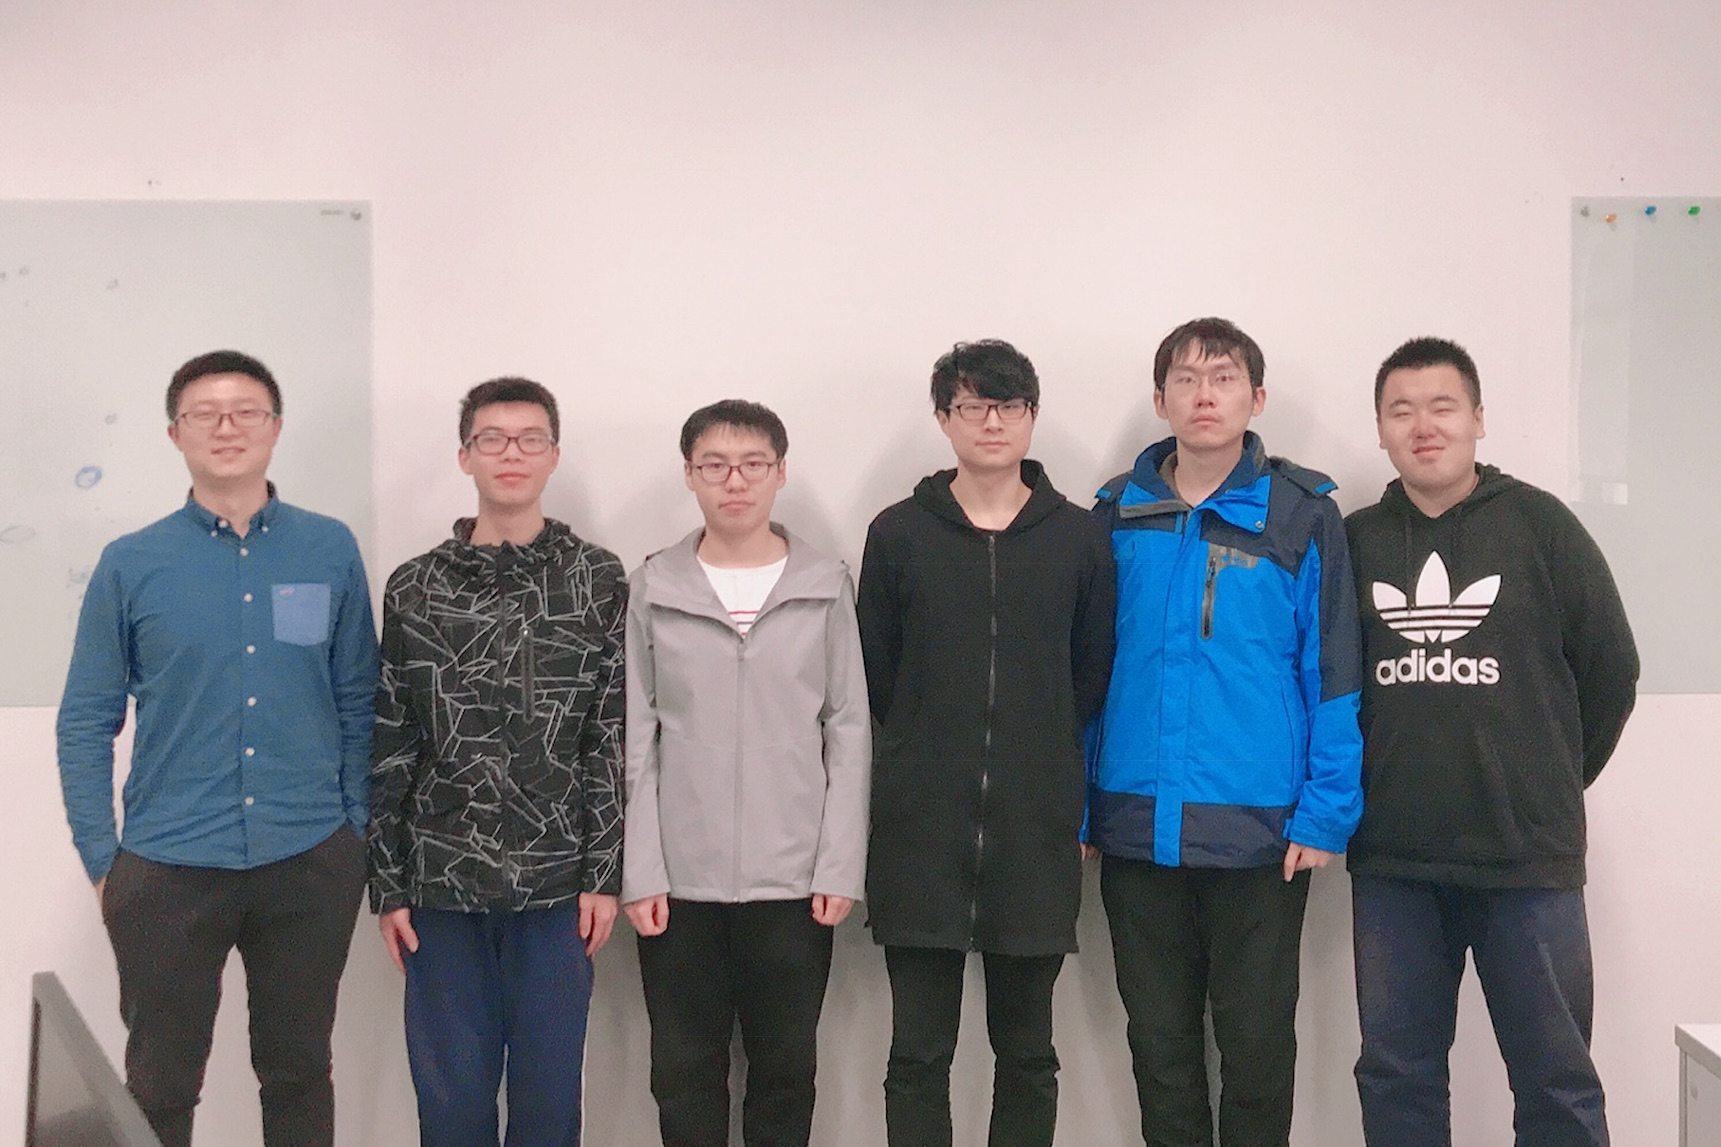
\includegraphics[width=12cm]{group.jpg}
\caption{Our Team Members}
\label{fig:Our Team Members}
\end{figure}


\subsection{Team Slogan}

\textbf{If you think you can, you can.}




\section{HPC System Design}

\par Objective: Design a system to achieve the best computing performance under 3,000-watt power consumption. Specify your system’s software and hardware configuration and interconnection. Describe the power consumption, evaluate the performance, and analyze the advantages and disadvantages of your proposed architecture.

\subsection{Hardware Environment}

\par Our proposed system is based on the Inspur NF5280M5 server following instructions and recommendations. The components and power consumption estimation listed in the table below.

\begin{table}[h]
\centering
\caption{Hardware Configuration In Our Design}\label{tab:Hardware Configuration In Our Design}
\begin{tabular}{cclc}
\toprule
Item & Name & Configuration & Power Estimation\\
\midrule

Server & \tabincell{c}{Inspur \\ NF5280M5} & \tabincell{l}{CPU : Intel Xeon Platinum 8176M $\times$ 2\\
		 \qquad \quad ($2.1GHz \sim 3.8GHz$, \quad 28 Cores)  \\ 
		 \qquad \quad TDP : 165 $W$ $\times$ 2\\
		GPU : NVIDIA TESLA V100 $\times$ 4\\
		\qquad \quad TDP : 250 $W$ $\times$ 4\\
		Memory: 64GB , DDR4 , 2400$MHz$ $\times$ 12\\
		\qquad \quad TDP : 6 $W$ $\times$ 12 \\  
		Hard Disk: Intel SSD Pro 7600p $\times$ 24\\
		\qquad \quad (512GB, M.2, PCIe 3.0x4) \\
		\qquad \quad TDP : 50 $mW$ $\times$ 24 } & \tabincell{c}{One Node : $1403.2W$\\ (2 Node in System)} \\

\midrule
\tabincell{c}{HCA \\ Card} & FDR & \tabincell{l}{InfiniBand Mellanox ConnectX-3 HCA \\card, Single port, QSFP, FDR IB} & \tabincell{c}{One Node : 9 $W$ \\ (2 Node in System)} \\

\midrule

Switch &\tabincell{c}{FDR-IB \\ Switch} & \tabincell{l}{$SwitchX^{TM}$ FDR InfiniBand switch, 36 \\ QSFP port} & 130 $W$ \\

\midrule

Cable &\tabincell{c}{InfiniBand \\ cable} & \tabincell{l}{InfiniBand FDR optical fiber cable, QSFP \\port, cooperating with the InfiniBand \\switch for use} & NaN \\

\bottomrule
\end{tabular}
\end{table}

\par Within the power limitation of 3000 Watts, the configuration can be used.

\par Through practical experience, it is found that accommodating more computing resources as much as possible in a single node is more conducive to improving the performance/power ratio of the entire HPC platform. At the same time, the huge I/O overhead due to network transmission can be minimized to achieve Maximizing performance under 3000-watt power limitations. In addition, CUDA-based GPGPUs have far greater parallel computing power than CPUs with the same power consumption. Based on this, our design criteria is to make full use of the resources of a single node as much as possible. In the whole system, we use two NF5280M5 servers based on the configuration shown in the table \ref{tab:Hardware Configuration In Our Design}. The theoretical power consumption of the entire platform is 2954.4 KW. When calculating the CUGPU-based GPGPU computing performance only, theoretical single-precision floating-point performance can reach 56 Tflops. 

\par In each node, we make full use of the maximum memory capacity supported by the Intel Xeon Platinum 8176M Processors and use a single 64GB DDR4-ECC memory to increase the memory capacity as much as possible so as to use the high-speed access performance of memory to reduce system I/O bottlenecks. We use 4 blocks. On the premise of the same power consumption, the NVIDIA TESLA V100 GPU enhances the performance of the system in scenarios such as deep learning. At the same time, we use 24 NVME-based SSDs to form a RAID array to provide more than 10 GB/s of disk I/O. Throughput.

\par In the connection part of the two nodes in the system, we connect through 16 linked InfiniBand methods to achieve a data exchange speed of up to 8 GB/s between the two computing nodes. At the same time, the master node is accessed through the ordinary Ethernet connection for the environment configure and monitoring. The overall structure of the system is shown in Figure \ref{fig:System Overall Structure}

\begin{figure}[!h]
\small
\centering
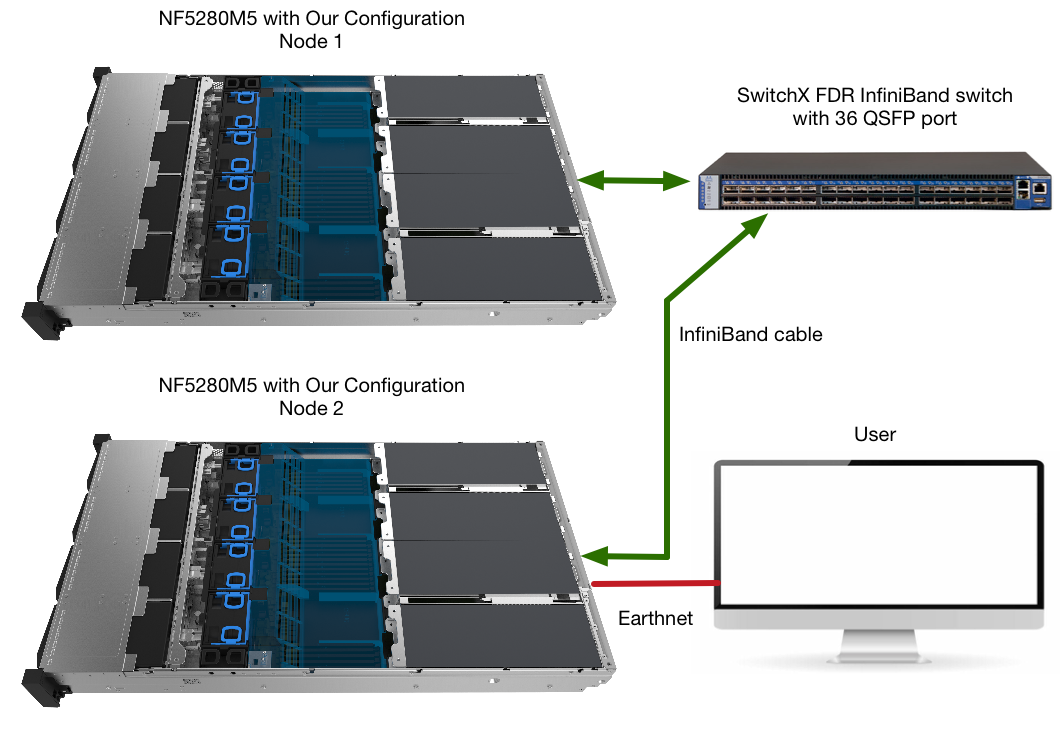
\includegraphics[width=12cm]{systemDesign.png}
\caption{System Overall Structure}
\label{fig:System Overall Structure}
\end{figure}




\subsection{Software Environment}


\begin{itemize}
	\item Operating System: RedHat Linux
	\item Development Kit
	\begin{itemize}
		\item Intel C++/Fortran Compiler
		\item Intel MKL Math Core Library
		\item GNU series compiler
		\item GNU gprof
		\item Intel VTUNE
	\end{itemize}
	\item Operating environment
	\begin{itemize}
		\item MVAPICH2, OpenMPI and MPICH Parallel Environment
		\item HPC, Hadoop and Spark Computing Environment
		\item NFS and RamDisk 
	\end{itemize}
	\item Cluster Monitoring and Scheduling System 
	\begin{itemize}
		\item PBS
		\item OOZIE
	\end{itemize}
\end{itemize}



\section{HPL Test}


\subsection{Hardware Platform and Theoretical Performance}

We use the single-node dual-circuit computing platform for HPL tuning in this question, for our hardware platform:

\begin{itemize}
	\item CPU : Intel Xeon E5460 (2.66$GHz$, 8C16T)  $\times$ 2 
	\item Memory : 8GB DDR3-ECC 1600$MHz$ $\times$ 18
\end{itemize}



According to Intel official data \upcite{bib:E5640}, we calculated the theoretical performance of our hardware platform to be $2.66 \times 16 \times 2 = 85.12 Gflops$

\subsection{Software Platform}

\par For baseline, we use the intel HPL-2.1 in round 0. Then we use the recompiling version HPL-2.2 for optimization. The software platform is shown flow: 

\begin{itemize}
	\item \textbf{System} : Ubuntu 16.04.3 LTS
	\item \textbf{Compiler \& MKL} : Intel Parallel Studio XE 2018.1
	\item \textbf{Round 0} : Intel original HPL-2.1
	\item \textbf{Round 1-4} : Recompiling version of HPL-2.2
\end{itemize}

\subsection{Optimization Process}

\par We first tested the calculation speed of baseline in round 0. According to Intel and HPL related documents \upcite{bib:HPL1, bib:HPL2, bib:HPL3} the possible optimal parameters were calculated at $N = 130000$, $NB = 120$, $P = 4$, $Q = 4$. Afterwards, we find the optimal parameters by adjusting the four different parameters.

\par According to the consulted documents, we conclude that the parameters that have obvious influence are N, NB, P, and Q. According to the formula \ref{HPL-N}, the theoretical maximum performance value is $N=135092$. The NB value ranges from $32\sim256$. .

\begin{equation}
	\label{HPL-N}
	N \times N \times 8 = 80\% \times MaxMemorySize
\end{equation}


\subsubsection{Round 0}

\par In round 0, we use the default Intel HPL environment for testing. The main parameters are shown in the following table \ref{tab:Parameters in Round 0 for Baseline}:

\begin{table}[h]
\centering
\caption{Parameters in Round 0 for Baseline}\label{tab:Parameters in Round 0 for Baseline}
\begin{tabular}{ll}
\toprule
Parameters & Content\\
\midrule
Ns & 130000 \quad 102400 \quad 150000 \\
NBs & 110 \quad 120 \quad 130 \\
Ps & 4\\
Qs & 4\\
\bottomrule
\end{tabular}
\end{table}

\par In this round, the computing power of our computing platform that we tested floats around 38 Gflops. Some of the test results are shown in the following table \ref{tab:Part of Log in Round 0}. The final log files are detailed in the appendix.

\begin{table}[h]
\centering
\caption{Part of Log in Round 0}\label{tab:Part of Log in Round 0}
\begin{tabular}{cccc}
\toprule
Column & Fraction & Kernel & Mflops\\
\midrule
022110 & 0.170 & 37958.81 & 38495.56\\
022770 & 0.175 & 38081.28 & 38479.87\\
023430 & 0.180 & 38564.32 & 38480.45\\
024090 & 0.185 & 37967.46 & 38464.89\\
024750 & 0.190 & 38317.15 & 38461.91\\
025410 & 0.195 & 38406.03 & 38459.64\\
026070 & 0.200 & 37941.81 & 38447.85\\
\bottomrule
\end{tabular}
\end{table}


\subsubsection{Round 1}

\par In the current round, we adjusted the values of N, NB, P, and Q within a certain range, and conducted tests to determine the actual performance under different parameters.

\textbf{Influence of different NB values}


\par We tested the computational performance of $NB = 2, 10, 20, 40, 80, 160, 320, and 640$ for the two cases $N = 4096$ and $N = 20480$. As shown in figure  \ref{fig:Performance Changes with N = 4096 r1}, the performance curve for different NB values when $N = 4096$. As shown in figure \ref{fig:Performance Changes with N = 20480 r1}, the performance curve for different NB values when $N = 20480$. Here $P=2$ , $Q=8$. It can be seen that as the NB value becomes larger, the performance increases first and then decreases, and there is a peak. When $NB=80$ and $NB=160$, the calculation performance is equivalent.


\begin{figure}[htbp]  
\begin{minipage}[t]{0.5\textwidth}
\centering  
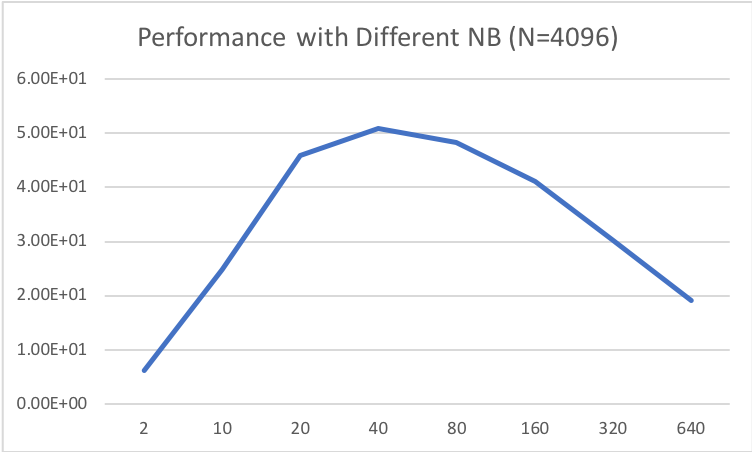
\includegraphics[width=\linewidth]{HPL_1_NB_1.png} \\
\caption{Performance Changes with N = 4096} \label{fig:Performance Changes with N = 4096 r1}
\end{minipage}
\hspace{1ex}
\begin{minipage}[t]{0.5\textwidth}  
\centering  
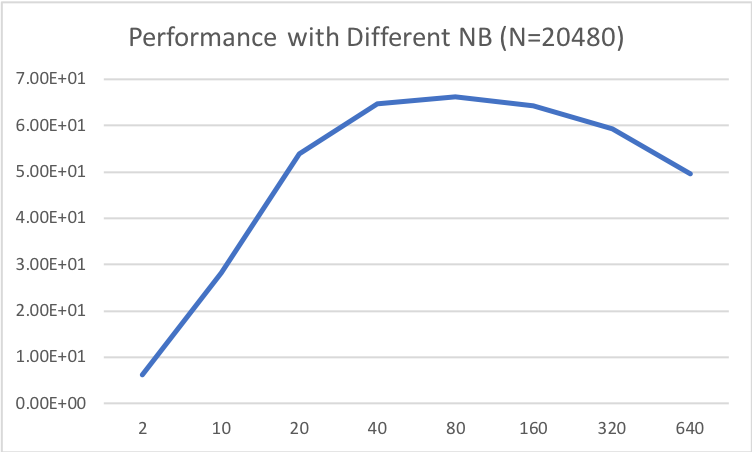
\includegraphics[width=\linewidth]{HPL_1_NB_2.png}\\
\caption{Performance Changes with N = 20480}  \label{fig:Performance Changes with N = 20480 r1}
\end{minipage}  
\end{figure} 


\textbf{Influence of different N values}

\par We tested the computational performance of $N = 2048, 4096, 10240, 20480, 40960, 102400 $ in two cases $NB = 20$ and $NB = 160$. As shown in figure \ref{fig:Performance Changes with NB = 20 r1},the performance curve of different N values at  $NB = 20$ . As shown in figure \ref{fig:Performance Changes with NB = 160 r1}, the performance curve for different N values when $NB = 160$. Here $P=2$, $Q= 8$. It can be seen that the performance increases gradually as the value of $N$ increases.

\begin{figure}[htbp]  
\begin{minipage}[t]{0.5\textwidth}
\centering  
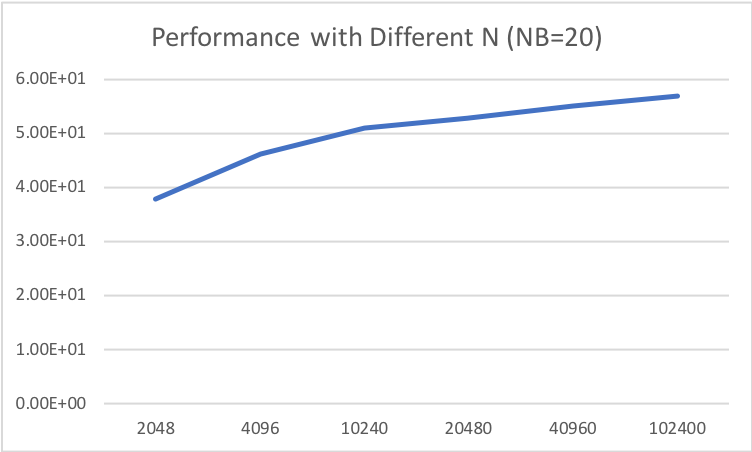
\includegraphics[width=\linewidth]{HPL_1_N_1.png} \\
\caption{Performance Changes with NB = 20} \label{fig:Performance Changes with NB = 20 r1}
\end{minipage}
\hspace{1ex}
\begin{minipage}[t]{0.5\textwidth}  
\centering  
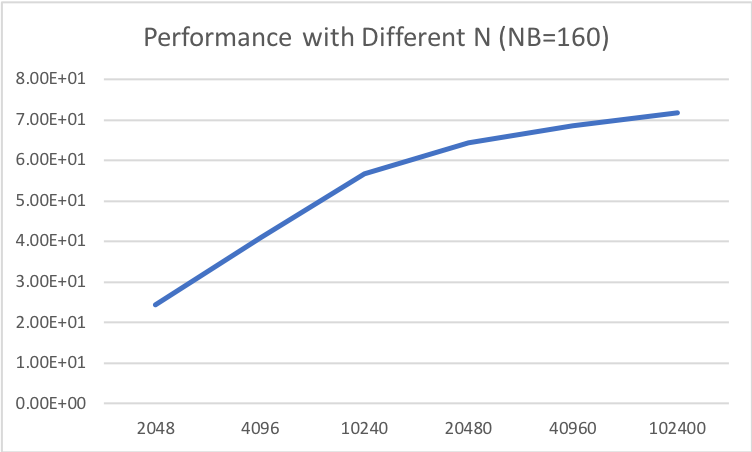
\includegraphics[width=\linewidth]{HPL_1_N_2.png}\\
\caption{Performance Changes with NB = 160}  \label{fig:Performance Changes with NB = 160 r1}
\end{minipage}  
\end{figure} 

\textbf{Influence of different $P \times Q$ values}

\par We have tested $NB=20$, $NB=160$ and $N=4096$, and $N=20480$. $P\times Q = 1 \times 16,2 \times 8,4 \times 4, 2 \times 4,8 \times 2,$ Computational performance of these five cases. As shown in figure \ref{fig:Performance Changes with PQ N4096 r1}, for $NB = 20$ different $N$ and $P \times Q$ value performance changes Curve. As shown in figure \ref{fig:Performance Changes with PQ N20480 r1}, the performance curve of different $N$ and $P \times Q$ values for $NB = 160$.


\begin{figure}[htbp]  
\begin{minipage}[t]{0.5\textwidth}
\centering  
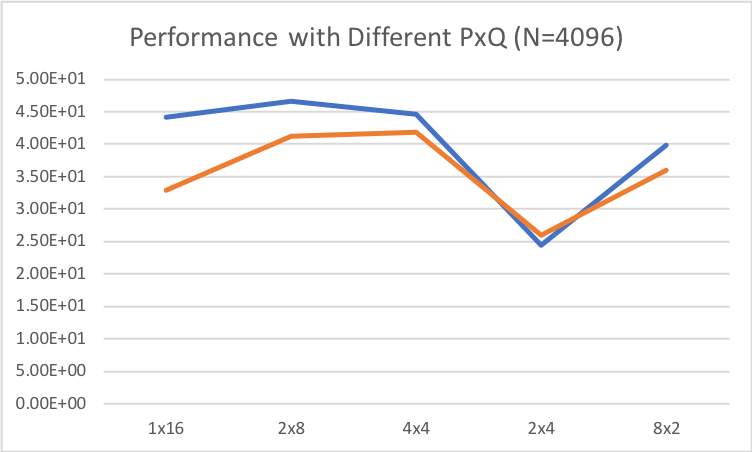
\includegraphics[width=\linewidth]{HPL_1_PQ_1.png} \\
\caption{Performance Changes with $P\times Q$ (N = 4096)} \label{fig:Performance Changes with PQ N4096 r1}
\end{minipage}
\hspace{1ex}
\begin{minipage}[t]{0.5\textwidth}  
\centering  
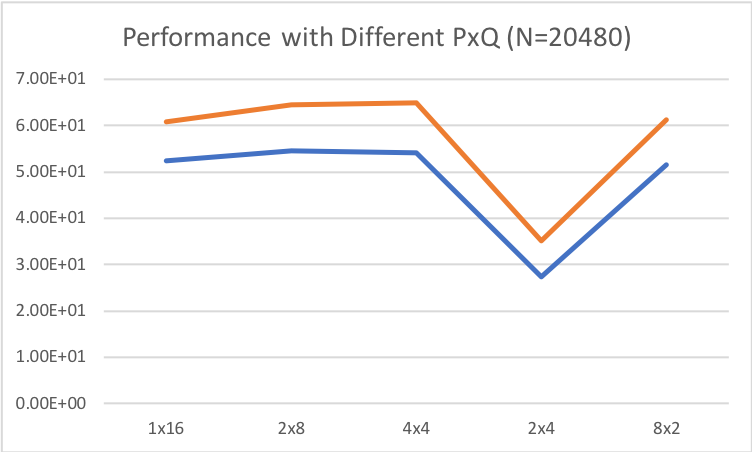
\includegraphics[width=\linewidth]{HPL_1_PQ_2.png}\\
\caption{Performance Changes with $P\times Q$ (N = 20480)}  \label{fig:Performance Changes with PQ N20480 r1}
\end{minipage}  
\end{figure} 

\par The orange line represents $NB=20$ and the blue line represents $NB=160$. Through analysis, it can be seen that $P \times Q$ can optimize performance at $4\times 4$.

\subsubsection{Round 2}

\par Through Round 1's analysis, we found that the parameter that has the greatest impact on performance is $NB$. When $P\times Q = 4 \times 4$, the best performance occured. Therefore, in this round, we selected $N=40960$, $P\times Q = 4 \times 4$, and tested the calculations for $NB = 80, 160, 320, and 640$. Performance (as shown in figure \ref{fig:Performance Changes r2}).



\subsubsection{Round 3}

\par Based on the previous round of testing, we determined the range of NB's value to $80 \leqslant NB \leqslant 240$, and tested the calculation performance for $NB = 80, 120, 160, 240$ (as shown in figure \ref{fig:Performance Changes r3}).



\begin{figure}[htbp]  
\begin{minipage}[t]{0.5\textwidth}
\centering  
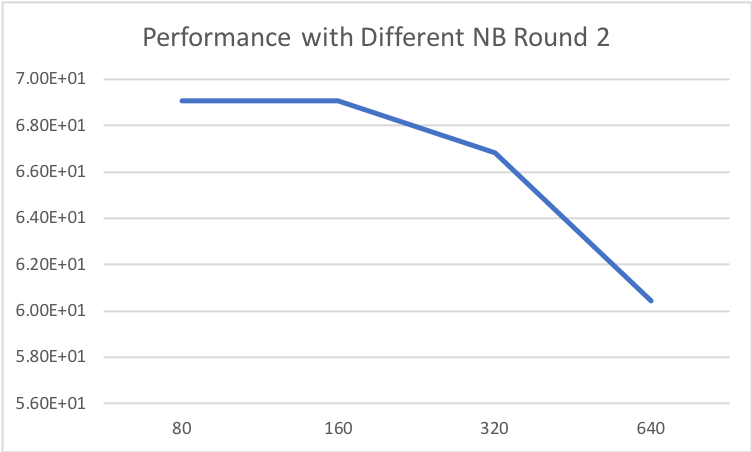
\includegraphics[width=\linewidth]{HPL_R2.png} \\
\caption{Performance Changes in Round 2} \label{fig:Performance Changes r2}
\end{minipage}
\hspace{1ex}
\begin{minipage}[t]{0.5\textwidth}  
\centering  
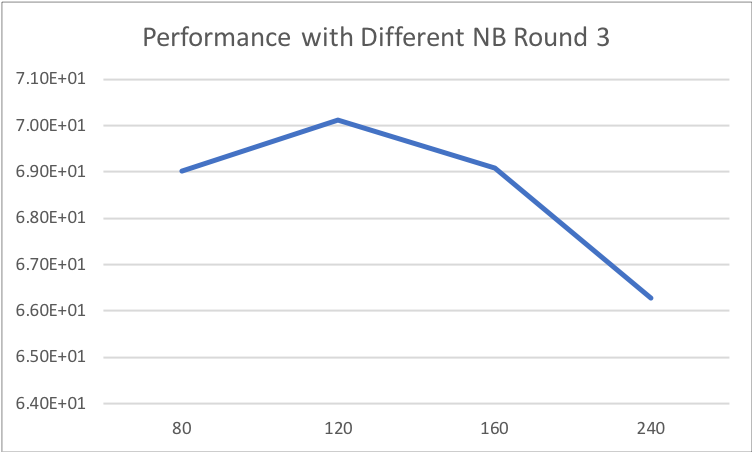
\includegraphics[width=\linewidth]{HPL_R3.png}\\
\caption{Performance Changes in Round 3}  \label{fig:Performance Changes r3}
\end{minipage}  
\end{figure} 


\subsubsection{Round 4}

\par Based on the previous round of testing, we set the NB's value range to $100 \leqslant NB \leqslant 140$. We tested the performance of calculations for $NB = 100,110, 120,130,140$ (as shown in figure \ref{fig:Performance Changes in Round 4}).

\begin{figure}[!h]
\small
\centering
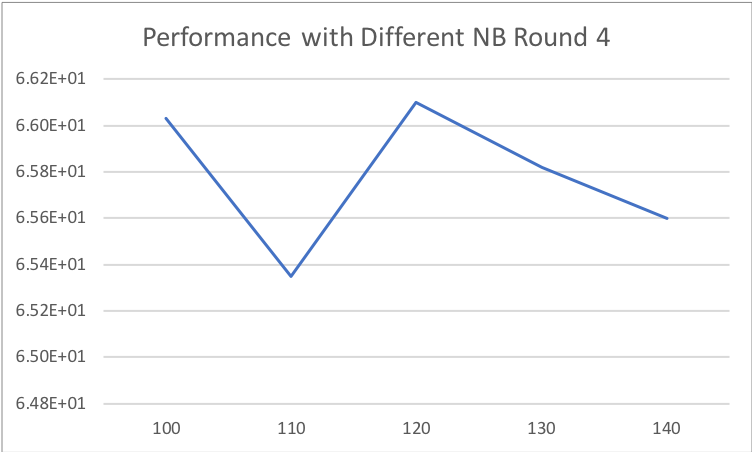
\includegraphics[width=12cm]{HPL_R4.png}
\caption{Performance Changes in Round 4}
\label{fig:Performance Changes in Round 4}
\end{figure}


\subsection{Summary}

\par In the HPL optimization, we consulted the document and parameter optimization. By analys the profiling result against xhpl, we found that 75\% time of the time was spent on one function of intel MKL, to be more specific, it's the code segment between 0x6c5600 and 0x6c5968 of libmkl\_mc3.so(show in figure \ref{fig:Profiling of HPL Start}, \ref{fig:Profiling of HPL End}).


\begin{figure}[!h]
\small
\centering
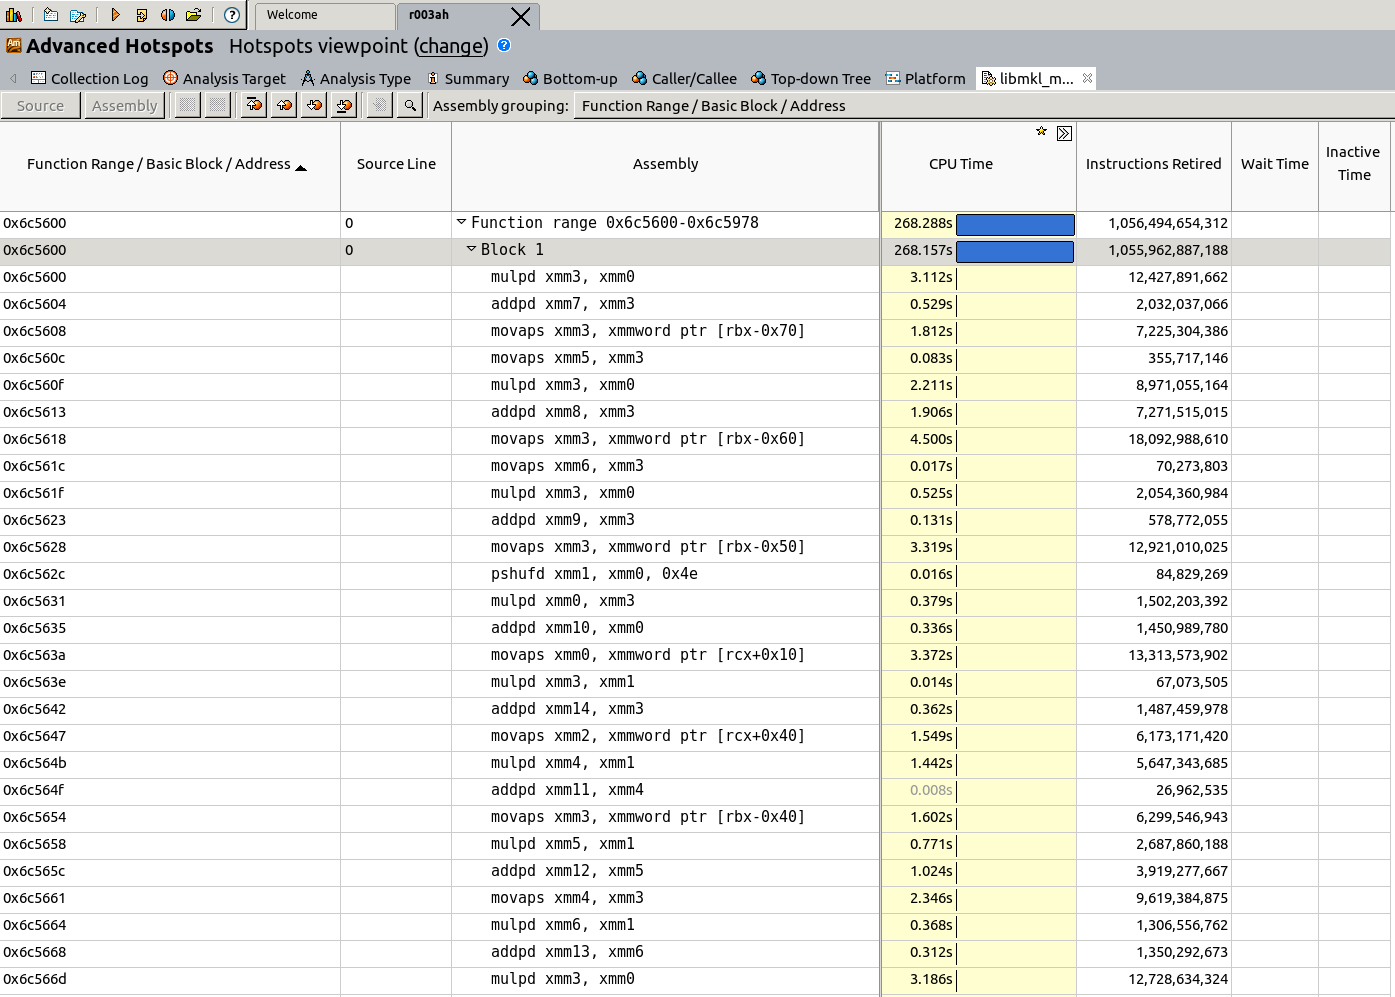
\includegraphics[width=14cm]{hpl_start.png}
\caption{Profiling of HPL Start}
\label{fig:Profiling of HPL Start}
\end{figure}

\begin{figure}[!h]
\small
\centering
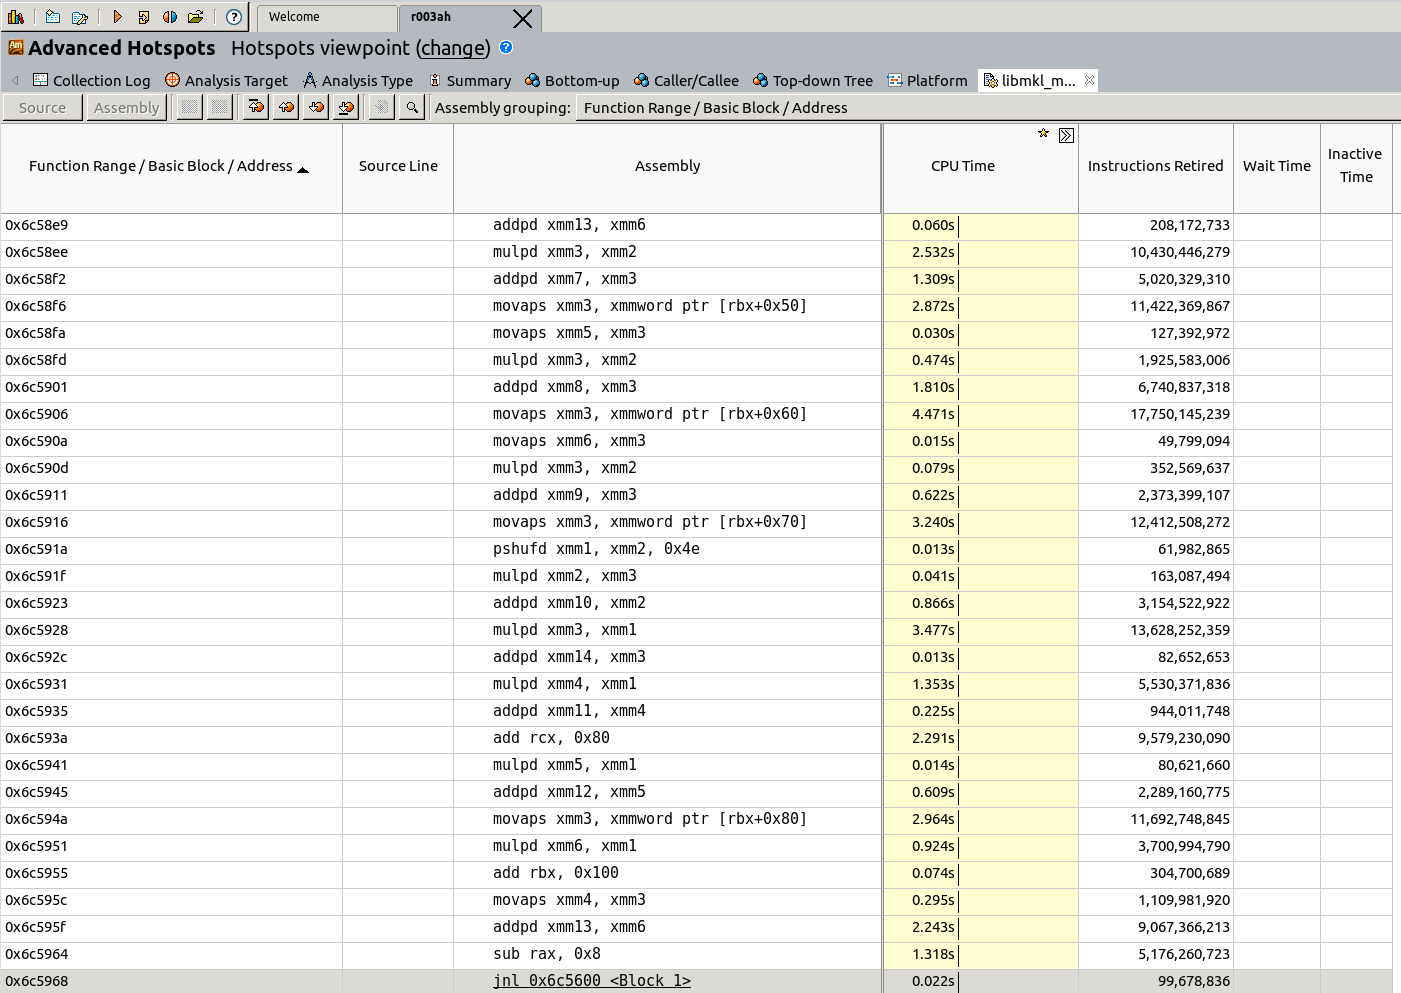
\includegraphics[width=14cm]{hpl_end.png}
\caption{Profiling of HPL End}
\label{fig:Profiling of HPL End}
\end{figure}




\par However, we failed to optimize this segment of code because it seems like to have been optimized well. We tended to optimize it by updating the instruction set to SSE4.2 but failed to find a instruction which works. Nor did we find the source code of intel MKL so we can recompile the library.

\par Finally determined that the computing performance is positively correlated with the value of N (before $N\leqslant 102400$), and the theoretical optimal value is 135093. The actual optimal value is: 200000. The calculation performance is positively correlated with the value of NB (before $NB \leqslant 160$), and the performance at $NB=80$ and $NB=160$ is equivalent, and the resulting optimal value is 120. $P\times Q = 4 \times 4$ is the value when the performance is optimal. The optimal performance is that it reaches the theoretical performance limit with 84.35\%. On our test platform, the optimal parameters are: $N = 20000$, $NB = 120$, $P = 4$, $Q = 4$. The best performance is $71.8Gflops$.

\section{HPCG Test}

\subsection{Hardware Platform}

\begin{itemize}
	\item CPU : Intel Xeon E5 2660v4 (2.0$GHz$, 14C28T) $\times$ 2 
	\item Memory : 32GB DDR4-ECC 2400 $MHz$ $\times$ 2
	\item GPU : Tesla K80 $\times$ 4
	\item Disk : HDD Driver 1TB 
\end{itemize}


\subsection{Software Platform}

\begin{itemize}
	\item \textbf{System} : Ubuntu 16.04.3 LTS
	\item \textbf{HPCG} : HPCG 3.1 binary compiled against CUDA 8.0.61
	\item \textbf{MPI} : Open MPI 1.10.2
	\item \textbf{Complier} : GCC 4.8.5
\end{itemize}

\subsection{Summary}

\par HPCG is designed as a different measure of HPC from HPL. 


\par We setup the environment for HPCG firstly. To compile OpenMPI with CUDA, we configured the source code of openmpi-1.10.2 with option "--with-cuda=/usr/local/cuda-8.0".

\par By comparing through results of different parameters(show in table \ref{tab:HPCG Test Log}), we found that the performing is best when CPU cores = GPU cores.


\begin{table}[h]
\centering
\caption{HPCG Test Log}\label{tab:HPCG Test Log}
\begin{tabular}{cccc}
\toprule
Process Grid	& Local Domain	& Final Performance (GF) \\
\midrule
1$\times$1$\times$1	&128$\times$128$\times$128	&26.7\\
2$\times$1$\times$1	&128$\times$128$\times$128	&56.2\\
2$\times$2$\times$1	&256$\times$256$\times$256	&109.3\\
2$\times$2$\times$1	&128$\times$128$\times$128	&108\\
2$\times$2$\times$2	&128$\times$128$\times$128	&103.4\\
4$\times$2$\times$2	&128$\times$128$\times$128	&101.2\\
\bottomrule
\end{tabular}
\end{table}

\par Since this is a binary release, optimization on the binary itself is considerably difficult. So we didn't optimize that.

\section{The RELION Test}

\subsection{Hardware Platform}

\begin{itemize}
	\item CPU : Intel Xeon E5 2660v4 (2.0$GHz$, 14C28T) $\times$ 2 
	\item Memory : 32GB DDR4-ECC 2400 $MHz$ $\times$ 2
	\item GPU : Tesla K80 $\times$ 4
	\item Disk : HDD Driver 1TB 
\end{itemize}


\subsection{Software Platform}

\begin{itemize}
	\item Ubuntu 16.04.3 LTS
	\item CUDA 8.0.61
	\item Open MPI 1.10.2
	\item Relion 2.1 Stable
\end{itemize}


\subsection{Parameter Tuning}





\par In this question, we determine that the parameter adjustment is mainly based on the estimating initial noise spectra of STEP1 (Class2D), estimating accuracies in the orthotropy assignment and iteration1 (a total of 25 iterations), and the operating speed, CPU efficiency, and GPU efficiency.


\par Firstly, when assigning the GPU to the MPI process, the default settings are used. The number of MPI processes must match 4n+1, 1 is the master process that is responsible for sending and receiving, and the rest is the slave process (responsible for operations).

\par Secondly, we tried to adjust the number of MPI processes, the total number of threads. But through actual testing found that the effect of this adjustment is not significant. Therefore choose to use 25 MPI processes, each process corresponds to a thread, each card is responsible for 6 MPI process.

\par Thirdly, trying to adjust the compiler parameters. When using the default cmake (intel compiler) compilation parameters, if you use 25 processes, half of the CPU usage is too low (less than 50\%), the GPU also Only reach 80~90W power. If you use 5 processes, CPU usage can be greatly improved, but the calculation speed is extremely low. After adding the O2 compiler parameters, the speed of the three steps can be increased by about one time. At the same time, the O3 compiler parameters are analyzed, and the actual results are not significant.

\par Finally, the intel compiler includes the parallel parameter by default, and can automatically optimize some loops that can be parallelized. After adding, the running time of estimating initial noise spectra is shortened from $8 \sim 9$ seconds to 5 seconds, and there is a significant improvement.

\par The final optimal operating parameters for STEP1 are as follows:

\begin{lstlisting}
mpirun -n 25 "which relion_refine_mpi" --gpu --o Class2D/job007/ --i particles.star --ctf --iter 25 --tau2_fudge 2 --particle_diameter 150 --K 100 --flatten_solvent --zero_mask --strict_highres_exp 8 --oversampling 1 --psi_step 12 --offset_range 5 --offset_step 2 --norm --scale
\end{lstlisting}

\subsection{Code Optimization}

\subsubsection{First Hot Point}

\par Though we could hardly find a better way like -O2, we have found something ably to better by checking the codes.When we use -O2 to faster the program on Estimating initial noise spectra, we know it could be hardly better on CPU.

\par So we try to use OpenACC to make the for loop paralleled better running on GPU.And we find a great number of for loops in the codes:fftw.h, fftw.cpp, mask.cpp, matrix1d.h, matrix2d.h. 

\par However, after adding the statements accompanied with their clause:

\begin{lstlisting}
#pragma acc kernels 
#pragma acc parallel 
\end{lstlisting}

\par we find that we could hardly configure the corresponding environment for OpenACC (We have tried GCC5.3.0,GCC6.1.0 and GCC7.1.0). So we're sorry for no results of it.

\subsubsection{Second Hot Point}

\par Another point is that, the marcos in multidim\_array.h and multidim\_array.cpp contains a lot of for loops.But we can't directly add the OpenACC codes in it or add it in front of the quote of the marcos (because the format of the for loop is illegal for OpenACC's optimizing).Our scheme is to rewrite the marcos, move the variables out or to a right place.

\subsubsection{Third Hot Point}

\par The 3rd point we have considered to better is that: the optimizing of MPI is based on the parallel of tasks rather than the parallel of calculations. That means, there are a lot of matrixs and FFT operations working on a serial state. At the beginning, we try to use OpenMP to greater the threads and better the efficiency. However, because of our poor hardware, the optimizing isn't evident (actually, we have make all the sources run for the codes). So the next step is to rewrite the logic of MPI's scheduling. However, then we are struggling with the build for OpenACC's environment and decline the time for this way.As a result, we didn't have enough time to achieve it.


\subsection{Answer Summary}

\par In this question, the first step and the second step are based on the combination of CPU + GPU computing method, the third step due to the computing platform, using only the CPU to calculate. 

\par The Baidu SkyDrive links to : \url{https://pan.baidu.com/s/1beTeVWpHKK1uIs_qAUywlg} .The key is : $nicp$.

\par The MD5 Code for answer's file is listing as flowing: 

\begin{itemize}
	\item \textbf{Step1.Class2D.tar.gz} : 7b64b0357f0dfec9a867438dfd3a605f
	\item \textbf{Step2.Class3D.tar.gz} : 305f41069e20232887ff2f9d8b724261
	\item \textbf{Step3.Refine3D.tar.gz} : 191b5ef232492a74ab346e411e2db68e
\end{itemize}


\subsubsection{Step I : Class 2D}

\par Open in relion\_maingui, import ".mrcs" file, node type is 2D micrograph movies (*.mrcs), press run now, press Display to open view. Get figure \ref{fig:Out Put in Step 1}.

\begin{figure}[!h]
\small
\centering
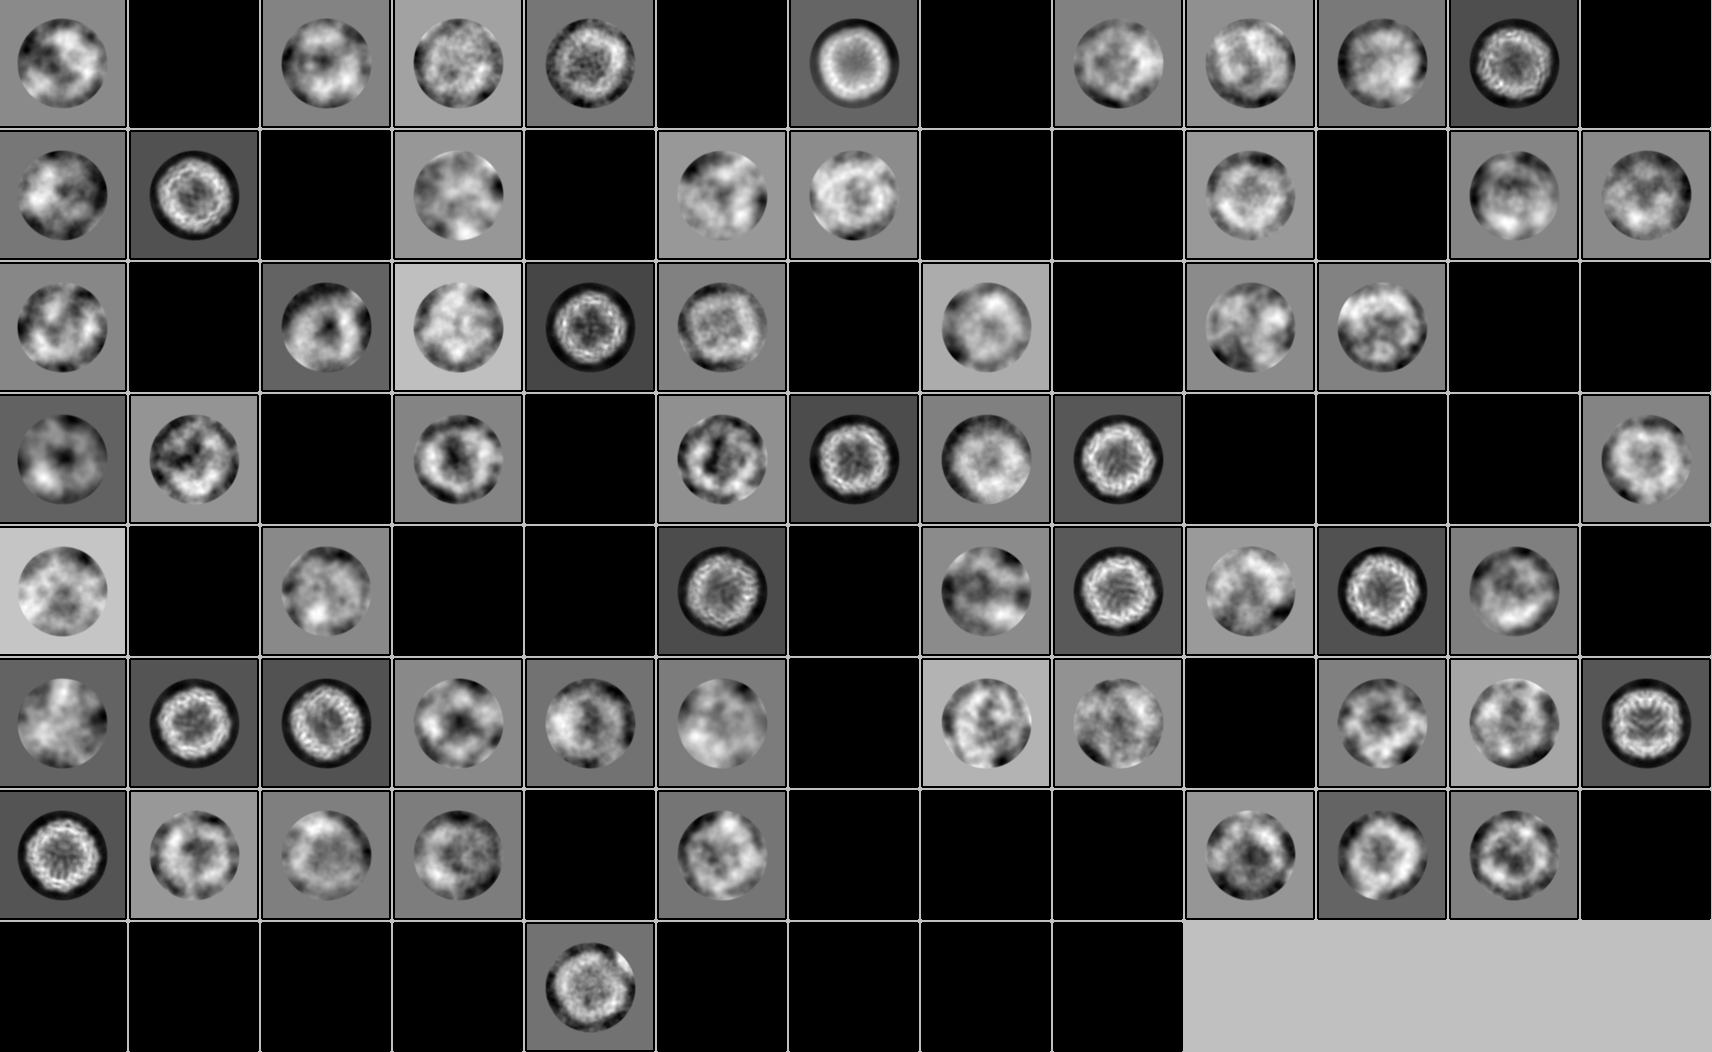
\includegraphics[width=10cm]{Relion1.png}
\caption{Out Put in Step 1}
\label{fig:Out Put in Step 1}
\end{figure}


\subsubsection{Step II : Class 3D}


\par Open in relion\_maingui, import ".mrc" file, node type is 3D reference (*.mrc), press run now, press Display to open the view. We select some pictures from the slice of the stereo image (show in figure \ref{fig:Part of Out Put in Step 2}).


\begin{figure}[htbp]  
\caption{Part of Out Put in Step 2} \label{fig:Part of Out Put in Step 2}
\centering
\begin{minipage}[t]{0.15\textwidth}
\centering  
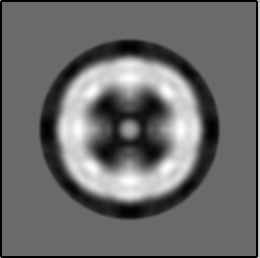
\includegraphics[width=\linewidth]{r1.png} \\
\end{minipage}
\hspace{1ex}
\begin{minipage}[t]{0.15\textwidth}  
\centering  
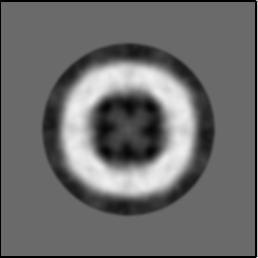
\includegraphics[width=\linewidth]{r2.png}\\
\end{minipage}  
\hspace{1ex}
\begin{minipage}[t]{0.15\textwidth}  
\centering  
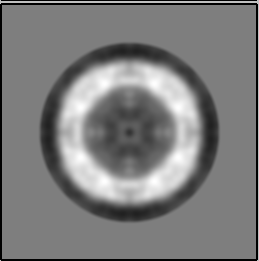
\includegraphics[width=\linewidth]{r3.png}\\
\end{minipage}  
\hspace{1ex}
\begin{minipage}[t]{0.15\textwidth}  
\centering  
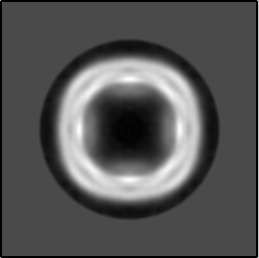
\includegraphics[width=\linewidth]{r4.png}\\
\end{minipage}  
\hspace{1ex}
\begin{minipage}[t]{0.15\textwidth}  
\centering  
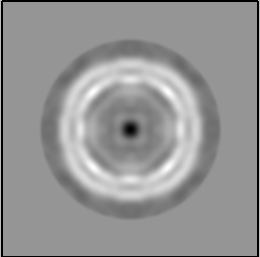
\includegraphics[width=\linewidth]{r5.png}\\
\end{minipage}  
\end{figure} 




\subsubsection{Step III : Refine 3D}

\par Use UCSF Chimera to adjust. Open the ".mrc" file, then set the step to 1 (connect the initial fractured graph), select level as 0.0272, Radius as 3.3, make the image as close as possible to the original, and then adjust the angle to get the desired image (show in figure \ref{fig:Out Put in Step 3}).


\begin{figure}[htbp]  
\caption{Out Put in Step 3} \label{fig:Out Put in Step 3}
\centering
\begin{minipage}[t]{0.45\textwidth}
\centering  
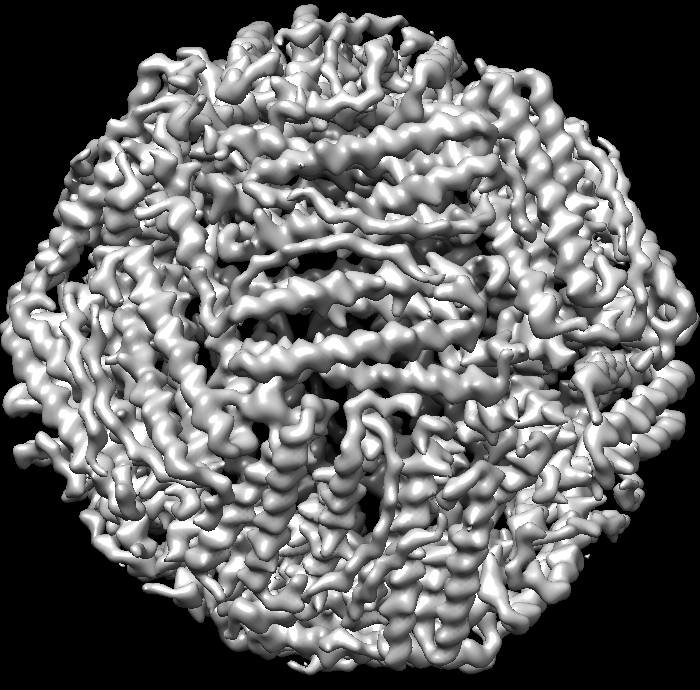
\includegraphics[width=\linewidth]{r6.png} \\
\end{minipage}
\hspace{1ex}
\begin{minipage}[t]{0.45\textwidth}  
\centering  
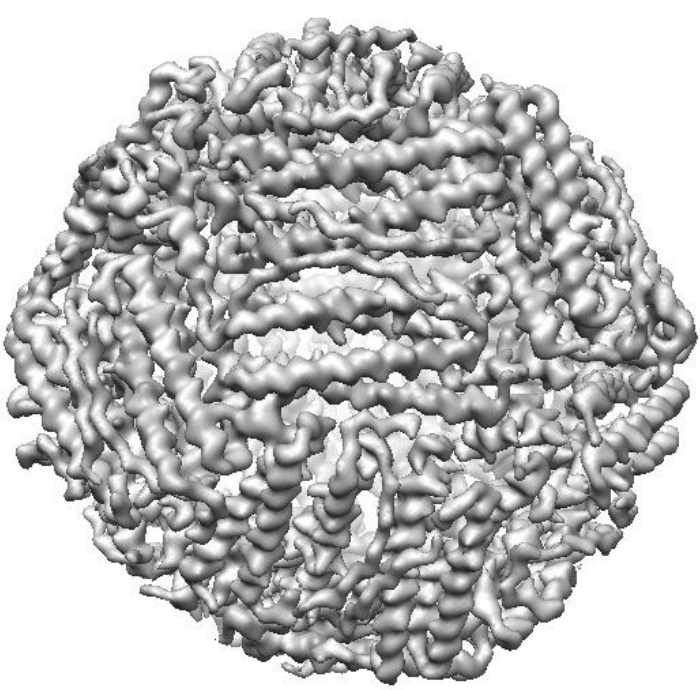
\includegraphics[width=\linewidth]{r7.png}\\
\end{minipage}  
\end{figure} 





\section{Answer Prediction for Search Query}

\subsection{Hardware Platform}

\begin{itemize}
	\item CPU : Intel Xeon E5 2660v4 (2.0$GHz$, 14C28T) $\times$ 2 
	\item Memory : 32GB DDR4-ECC 2400 $MHz$ $\times$ 2
	\item GPU : Tesla K80 $\times$ 4
	\item Disk : HDD Driver 1TB 
\end{itemize}


\subsection{Software Platform}

\begin{itemize}
	\item Ubuntu 16.04.3 LTS
	\item CUDA 8.0.61
	\item CNTK 2.4
\end{itemize}


\subsection{Summary}
\par We learned the usage of CNTK through the baseline code and its documentation, and designed a network with a variety of attention mechanisms. However, due to the constraints of our hardware, the training of the network with self-attention will be very slow so that we cannot adjust the effect of the network. We tried to run test on the MSMARCO dataset after training on the Stanford SQUAD dataset, but the results were worse than baseline. Finally, we used Bi-directional attention flow network architecture then adjust a variety of hyper-parameters and selected the best performing model on the validation set as our submission.

\par Part of the output is shown below (json format):


\begin{lstlisting}
{"query_id": 0, "answers": ["not"]}
{"query_id": 1, "answers": ["petroleum oil , natural gas , and coal . Fossil fuels , like coal , oil , and natural gas , provide the energy that powers our lifestyles and our economy ."]}
{"query_id": 2, "answers": ["The apothem of a regular polygon is a segment drawn the center of the polygon ( that is , the center of the circle which circumscribes the polygon ) to one side , such that it is perpendicular to the side ."]}
{"query_id": 3, "answers": ["$ 600 to $ 1400"]}
{"query_id": 4, "answers": ["Hardware is a comprehensive term for all of the physical parts of a computer , as distinguished from the data it contains or operates on , and the software that provides instructions for the hardware to acoomplish tasks ."]}
{"query_id": 5, "answers": ["a firm that provides service to its customers of outsourced ( or Third Party ) logistics services for part , or all of their supply chain management functions ."]}
{"query_id": 6, "answers": ["Contrary to the beliefs of those who advocate the legalization of marijuana , the current balanced , restrictive , and bipartisan drug policies of the United States are working reasonably well and they have contributed to reductions in the rate of marijuana use in our nation ."]}
{"query_id": 7, "answers": ["spiders , scorpions , ticks , mites , harvestmen , and their cousins ."]}
{"query_id": 8, "answers": ["southeastern Russia and the Jilin Province of northeast China ."]}
{"query_id": 9, "answers": ["$ 50 - 75"]}
{"query_id": 10, "answers": ["Proteus mirabilis is part of the normal flora of the gastrointestinal tract , and as a result the bacteria enters the urinary tract or infects medical equipment by the fecal route ."]}
\end{lstlisting}

See the appendix for complete results.


%% reference ----------------------->
\begin{thebibliography}{99}

\bibitem{bib:HPL1} \url{https://software.intel.com/en-us/articles/performance-tools-for-software-developers-hpl-application-note}

\bibitem{bib:HPL2} \url{https://bytefreaks.net/programming-2/}

\bibitem{bib:HPL3} \url{http://www.netlib.org/benchmark/hpl/faqs.html#blsize}
\bibitem{bib:E5640} \url{https://ark.intel.com}
\end{thebibliography}


%% reference over ----------------->

%% appendices data ----------------->
\begin{appendices}
\begin{itemize}
	\item HPL Log: \quad (path: ./HPL)
	\item HPCG Log: \quad  (path: ./HPCG)
	\item Answer Prediction For Search Query: \quad  (path: ./AnswerPrediction)
\end{itemize}
\end{appendices}

\end{document}

